
\chapter{Integral Reduction}
\label{sec:reduction:dimension}

The quantity  $\mathcal{A}$ of particles from a polygon $A$
to a polygon $B$,  can be computed
by integrating the individual dispersal function, $\phi(y-x)$,
over pairs  of points $(x,y)$, $x\in A$, $y\in B$,
see~Section~\ref{introduction} and Fig.~\ref{fig:int:geom:1}.

\begin{figure}[htbp]
  \subfigure[The first and second points of each pair can be
  chosen independently in  $A$ and
  $B$.]{\includegraphics[width=7.5cm]{VignetteDir/graphics/integral_geom_1.eps}}
  \subfigure[Consider all the pairs of points separated by 
  the same vector $t$ ($t$ is in bold on the figure). For a given $t$, 
  $x\in A$ and $x+t\in B$, if and only if  $x\in
  A\cap\left(B-t\right)$ (such $x$ and $x+t$ are joined here by blue
  segments; $A\cap\left(B-t\right)$ is represented by 
 the blue area).]{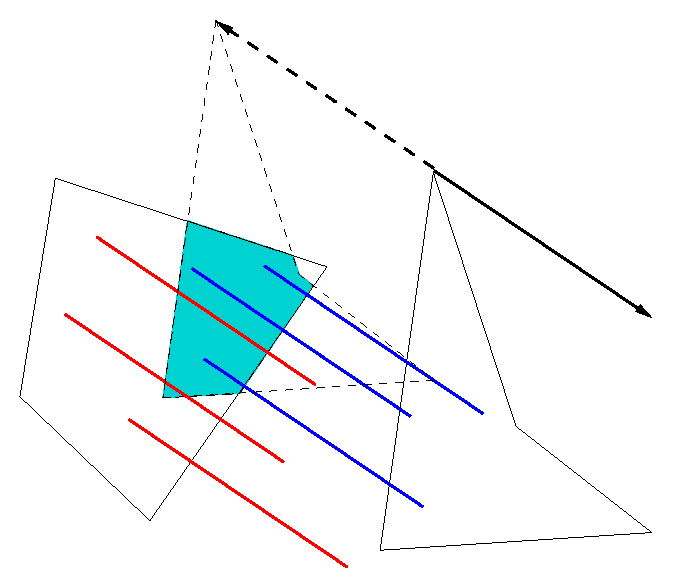
\includegraphics[width=7.5cm]{./VignetteDir/graphics/integral_geom_2.eps}}
  \caption{The quantity of particles from a polygon $A$
to a polygon $B$ is computed
by integrating the individual dispersal function
over all pairs of points $(x,y) \in A\times B$.
These pairs are represented here by segments.}
    \label{fig:int:geom:1}
\end{figure}

\medskip

Rather than scrolling through the pairs of points by choosing 
each member independently in  $A$ and $B$,
it is worth considering the pairs separated by the same vectors.
The dispersal function is constant on such subsets  of the pairs of
points.

\medskip
With the variable change $(x,y)\rightarrow (x,t=y-x)$, the set
\begin{equation*}
  \left\{y-x|x\in A, y\in B\right\}
\end{equation*}
can be written  $\check{A}\oplus B$ where $\check{A}=-A$
and $\oplus$ stands for the Minkowski sum.
The Minkowski sum of two sets $A$ and $B$ is simply the set obtained
by addition of the points of $A$ and $B$ (see
Fig.~\ref{fig:minkowski}). On the other hand, for each
vector $t\in \check{A}\oplus B$: 
\begin{equation*}
  x\in A, y=x+t\in B \Leftrightarrow x\in A\cap\left(B-t\right) 
\end{equation*}

\begin{figure}[htbp]
  \begin{center}
    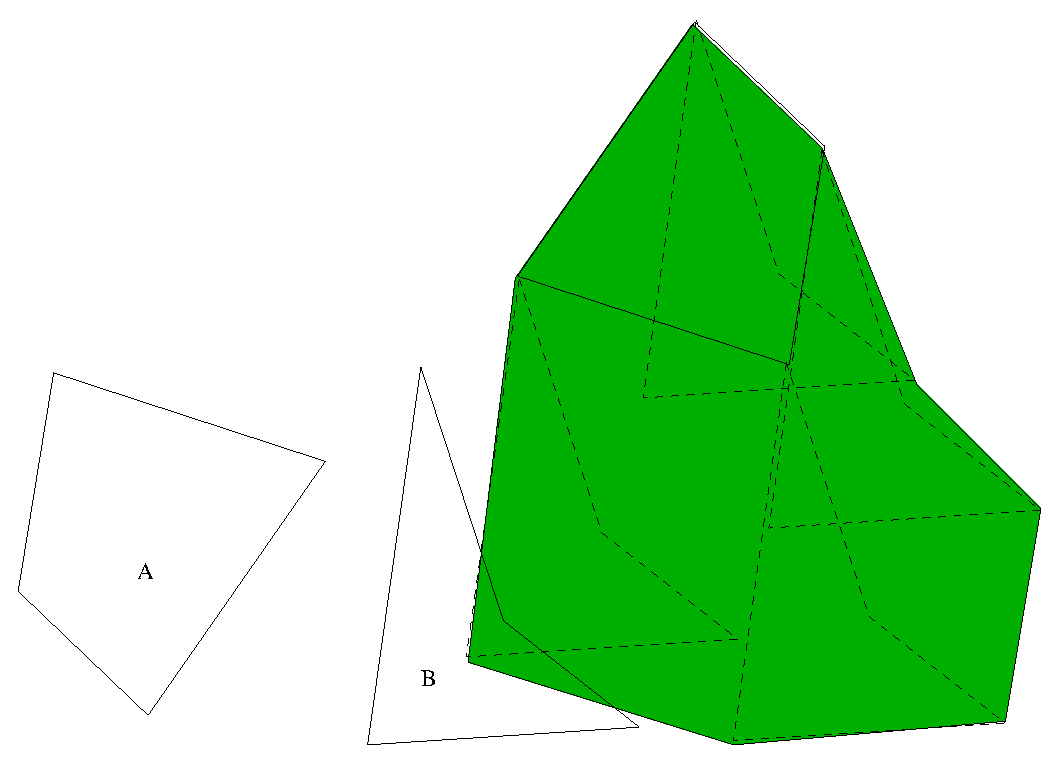
\includegraphics[width=10cm]{./VignetteDir/graphics/integral_geom_4.eps}
    \caption{The set of points $t=y-x$, where $x\in A$ and 
$y\in B$, is written $\check{A}\oplus B$. 
It is the set of points
covered by $B$ when the vertex $o$ is moved inside $\check{A}$.
Here, to simplify, the origin of the plan $o$ is
located on a vertex of  $B$.}
    \label{fig:minkowski}
  \end{center}
\end{figure}

Now, we can rewrite the integral $\A$ 
defined by the equation~\eqref{eq:def:A}:
\begin{eqnarray}
  \A &=& \int_{\check{A}\oplus B}\int_{A\cap \left(B-t\right)} 
  \phi(t) \,dx\,dt
\end{eqnarray}
as:
\begin{eqnarray}
  \A & = & \int_{\check{A}\oplus B}\int_{A\cap \left(B-t\right)} 
  \,dx\, \phi(t) \,dt.
\end{eqnarray}

The integral in $x$ is simply the area of $A\cap
\left(B-t\right)$, so:
\begin{equation}
  \label{lastexpression}
  \A = \int_{\check{A}\oplus B} \aire(A\,\cap\,(B-t)) \,\phi(t)
  \,dt 
\end{equation}

The computation of one of the two integrals has been replaced
by the computation of an area and of an intersection, the intersection
of  $A$ and a translation of $B$.
The calculation of~\eqref{lastexpression} has
proven to be faster than the one of~\eqref{eq:def:A}
\footnote{Time comparisons have been made by using the 
integration subroutines of the NAG~\cite{NAG} library,
D01FCF (adaptive integration, i.e where the evaluation 
spots depend
on the integrand), and  D01GCG (Korobov-Conroy method) 
on  real and simulated fields.}
So, it is the formula implemented in \verb+CaliFloPP+.


%%% Local Variables: 
%%% mode: latex
%%% TeX-master: t
%%% End: 
